\documentclass[10pt,compress,notheorems]{beamer}

%\usepackage{ucs}
\usepackage[utf8]{inputenc}
\usepackage[dark]{beamerthemesidebar}

%\usepackage{babel}
\usepackage{fontenc}
\usepackage{graphicx}
\usepackage{subfigure}
\usepackage{url}




\def \rr {$R_{t}\:$}

\author{Flávio Codeço Coelho and Luiz Max Carvalho}
\title{Estimating the Attack Ratio of Dengue Epidemics under Time-varying 
Force of Infection using Aggregated Notification Data}
\date{May 1st, 2015}
\institute [EMAp, FGV]{Applied Mathematics School,   Fundação Getúlio Vargas}


\logo{\includegraphics[width=\beamer@sidebarwidth]{./fb1.png}}
\begin{document}
 \begin{frame}
\titlepage
\end{frame}

\begin{frame}[fragile]
\frametitle{Summary}
\tableofcontents
\end{frame}

\section{Motivation}
\begin{frame}
\frametitle{Dengue Dynamics}
\begin{itemize}[<+->]
  \item Dengue is a Multi-Strain  vector-borne disease
  \item 4 major viral strains in circulation in Brazil
  \item Case-notification data is aggregated, i.e., does not discriminate 
serotype except for a handful of cases.
  \item It's a Seasonal disease, but recurrence pattern is hard to predict
  \item Vector population dynamics plays a major role in the modulation of 
incidence
  \item Imunological structure of the population is also a key factor, but is 
mostly unknown.
\end{itemize}
\end{frame}

\begin{frame}[fragile]
\frametitle{4 epidemics}
\begin{flushleft}
 \begin{figure}
\subfigure[2010]{\includegraphics[width=4.5cm, 
height=2.75cm]{./heatmap2010.jpg}}
  \subfigure[2011]{\includegraphics[width=4.5cm]{./heatmap2011.jpg}}
  \subfigure[2012]{\includegraphics[width=4.5cm]{./heatmap2012.jpg}}
  \subfigure[2013]{\includegraphics[width=4.5cm]{./heatmap2013.jpg}}
  \end{figure}
\end{flushleft}

\end{frame}

\subsection{Vector dynamics}

\begin{frame}
\frametitle{Environmental determinants}
\begin{block}{Vector dynamics}
\begin{itemize}[<+->]
 \item A. Aegypti population dynamics display marked seasonality
 \item Temperature, Humidity and rainfall are important factors
 \item Environmental stock of eggs
 \item Effects on mosquito reproduction are non-linear
 \item Delayed influence
\end{itemize}
\end{block}

\end{frame}


\section{Building blocks}

\subsection{Variable Force of Infection}
\begin{frame}
\frametitle{Effective Reproductive number(\rr)}
The effective reproductive number can be easily estimated from the incidence 
time-series, $Y_t$:
\begin{equation}
\label{eq:Rtestimate}
R_t = \left( \frac{Y_{t+1}}{Y_t}\right)^{1/n}
\end{equation}
Where $n$ is the ratio between the length of reporting interval and 
the mean generation time of the disease.
\begin{flushright}
 Nishiura et. al. (2010)
\end{flushright}
\end{frame}

\begin{frame}
\frametitle{\rr's uncertainty}
But what about the uncertainty about \rr\footnote{Coelho, FC and Carvalho, LM 
(Submitted)}?

We explore the approach of Ederer and Mantel\cite{mantel}, whose objective is 
to obtain 
confidence intervals for the ratio of two Poisson counts. 
Let $Y_{t} \sim Poisson(\lambda_t)$ and $Y_{t+1} \sim Poisson(\lambda_{t+1})$ 
and define $S = Y_{t} + Y_{t+1}$.
The authors note that by conditioning on the sum $S$
\begin{align}
\label{eq:binlike}
Y_{t+1} | S &\sim Binomial(S, \theta_t) \\
\theta_t &= \frac{\lambda_{t+1}}{\lambda_{t} + \lambda_{t+1}}
\end{align}
\end{frame}

\begin{frame}
\frametitle{\rr's Uncertainty}
Let $c_{\alpha}(\theta_t) = \{\theta_t^{(L)} , \theta_t^{(U)} \}$ be such that 
$Pr(\theta_t^{(L)}<\theta_t <\theta_t^{(U)}) = \alpha$.
Analogously, define $c_{\alpha}(R_t) = \{R_t^{(L)} , R_t^{(U)} \}$ such that 
$Pr(R_t^{(L)}<R_t<R_t^{(U)}) = \alpha$.

Ederer and Mantel (1974)~\cite{mantel} show that one can construct a $100\alpha 
\%$ confidence interval for \rr by noting that
\begin{equation}
\label{eq:confRt}
 R_t^{(L)} = \frac{\theta_t^{(L)}}{(1-\theta_t^{(L)})} \quad \text{and} \quad 
R_t^{(U)} = \frac{\theta_t^{(U)}}{(1-\theta_t^{(U)})}
\end{equation}
\end{frame}

\begin{frame}
\frametitle{\rr's Uncertainty}
Taking a Bayesian conjugate distribution approach, If we choose a
Beta conjugate prior with parameters $a_0$ and $b_0$ for the 
Binomial likelihood in (\ref{eq:binlike}), the posterior distribution for 
$\theta_t$ is
\begin{equation}
\label{eq:thetapost}
p(\theta_t| Y_{t+1}, S) \sim Beta(Y_{t+1} + a_0, Y_t + b_0)
\end{equation}
Combining equations~(\ref{eq:confRt}) and~(\ref{eq:thetapost}) 
tells us that the induced posterior distribution of $R_t$ is 
a Beta prime (or inverted Beta) with parameters $ a_1 = Y_{t+1} + a_0$ and $b_1 
=  Y_t + b_0$~\cite{dubey1970}.
The density of the induced distribution is then 
\begin{equation}
\label{eq:densityMantel}
f_P(R_t| a_1, b_1) = \frac{\Gamma(a_1 + b_1)}{\Gamma(a_1)\Gamma(b_1)} R_t^{a_1 
- 
1} (1 + R_t)^{-(a_1 + b_1)}
\end{equation}
Thus, the expectation of \rr is $a_1/(b_1 - 1)$ and its variance is 
$a_1(a_1 + b_1 - 1)/\left((b_1 - 2)(b_1 - 1)^2 \right) $.
\end{frame}



\begin{frame}
\frametitle{\rr's Uncertainty}
\begin{center}
\begin{figure}
  \includegraphics[width=9cm]{./rt_series.png}
\end{figure}
\end{center}
\end{frame}



\begin{frame}
\frametitle{\rr \emph{vs.} Temperature}
\begin{columns}
 \column{5cm}
\includegraphics[width=5cm]{./rt_min_t.png}

\includegraphics[width=5cm]{./rt_t24.png}
 \column{6cm}
\includegraphics[width=5cm]{./transmissao_temp.png}
\end{columns}
\end{frame}

\section{Modeling Dengue}
\subsection{Single-strain model}
\begin{frame}
\frametitle{Single Strain SIR}
Why not multi-strain? No Multi-strain data!!
\begin{align}
   \label{eq:model}
 \frac{dS}{dt} &= -\beta(t)SI \\     \nonumber
 \frac{dI}{dt} &= \beta(t)SI - \tau I&\\      \nonumber
 \frac{dR}{dt} &= \tau I&
\end{align}  
where $S(t) + I(t) + R(t) = 1 \: \forall\: t$. % \in [T_0, T_1]$. 


\end{frame}
\subsection{Variable Force of Infection}
\begin{frame}
\frametitle{Variable Force of Infection}
From \rr, we can define a force of infection which varies with time:
\begin{equation} 
 \label{eq:effbeta}
 \beta(t) = \frac{R_t\cdot\tau}{S}
\end{equation}
But how do we get the value of $S$? we need to estimate $S_0$.

\end{frame}


\section{Parameter estimation}
\subsection{Estimating $S_0$}
\begin{frame}
\frametitle{Estimating $S_0$}
Bayesian framework:
\begin{itemize}[<+->]
 \item Define priors for $S_0$ in the range (0,1)
 \item Samples from prior, calculate $\beta(t)$ and run the model
 \item calculate Likelihood of data given current parameterization
 \item Determine posterior probability of parameterization
\end{itemize}
\begin{equation}
 \label{eq:S0post}
 p(S_{0j}|\mathbf{Y_{j}}) \propto L(\mathbf{Y_{j}}|S_{0j}, R_t, m, \tau 
)\pi(S_{0j}) 
\end{equation}
\end{frame}

\begin{frame}[fragile]
\frametitle{Models \textit{vs} Data}
fiting the model to data (Rio de janeiro) to estimate $S_0$\footnote{Coelho 
FC et al., 2011}.

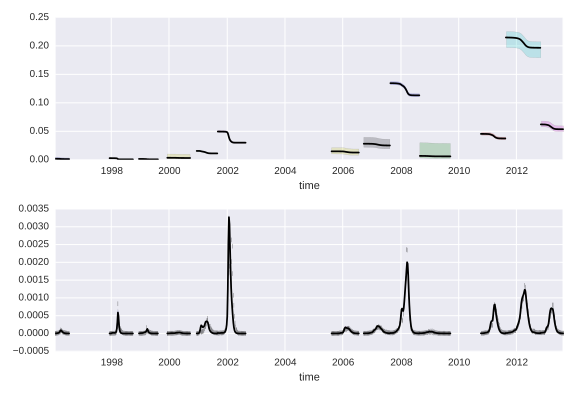
\includegraphics[width=\textwidth]{concat_SI.png}
 
 \begin{small}Posterior distribution for Susceptible (S) and infectious (I) 
individuous. Blue dots are data. \end{small}

\end{frame}

\subsection{Attack Ratio}
\begin{frame}
\frametitle{Attack Ratio}
Once we have $S_0$, we can caculate the attack ratio:
\begin{equation}
\label{eq:AR2}
 A_{j}=\frac{\sum Y_j}{S_{0j}}
\end{equation}
\end{frame}

\begin{frame}
\frametitle{Attack ratio}
\begin{table}[!ht]
\begin{tiny}\caption{
{\bf Median attack ratio and 95\% credibility intervals calculated according to 
(\ref{eq:AR2})}. 
Values are presented as percentage of total population. 
$^\dag$: Year corresponds to the start of the epidemic, however the peak of 
cases
may occur in the following year.
$^\ddag$: Susceptible fraction.
These results show considerable variation in AR between epidemics, consistent 
with
the accquiring and loss of serotype-specific immunity.}                          
                             \end{tiny}
\begin{center}
\begin{footnotesize}\begin{tabular}{c|c|c}
\hline
Year$^\dag$ & median Attack Ratio & $S_0^\ddag$ \\
\hline
1996 & 0.39 (0.17-0.54) & 0.00171(0.0012-0.0038)\\
1997 & 0.87 (0.74-0.87) & 0.00273(0.0027-0.0032)\\
1998 & 0.5 (0.49-0.5) & 0.00142(0.0014-0.0014)\\
1999 & 0.11 (0.037-0.2) & 0.00345(0.0018-0.01)\\
2000 & 0.25 (0.24-0.27) & 0.0155(0.015-0.016)\\
2001 & 0.48 (0.47-0.49) & 0.0495(0.048-0.051)\\
2005 & 0.15 (0.1-0.21) & 0.0147(0.01-0.021)\\
2006 & 0.11 (0.08-0.14) & 0.0281(0.022-0.037)\\
2007 & 0.15 (0.15-0.15) & 0.135(0.13-0.14)\\
2008 & 0.14 (0.031-0.31) & 0.00672(0.003-0.024)\\
2010 & 0.18 (0.17-0.19) & 0.0454(0.043-0.048)\\
2011 & 0.086 (0.082-0.094) & 0.215(0.2-0.23)\\
2012 & 0.14 (0.13-0.15) & 0.0621(0.058-0.068)\\
\hline
\end{tabular}\end{footnotesize}
\end{center}
\label{tab:AR}
\end{table}
\end{frame}
\begin{frame}[fragile]
\frametitle{References}
\begin{thebibliography}{10}
 \bibitem{nishiura}
Nishiura H, Chowell G, Heesterbeek H, Wallinga J (2010) {{T}he ideal reporting
  interval for an epidemic to objectively interpret the epidemiological time
  course}.
\newblock J R Soc Interface 7: 297--307.
%\bibAnnoteFile{nishiura}

\bibitem{pone2011}
Coelho FC, Code\c{c}o CT, Gomes MG (2011) {A} {B}ayesian framework for
  parameter estimation in dynamical models.
\newblock PLoS ONE 6: e19616.

\bibitem{pone2011}
Coelho FC, Carvalho, LM {E}stimating the Attack Ratio of Dengue 
Epidemics under Time-varying Force of Infection using Aggregated Notification 
Data
\newblock Arxiv. \url{http://arxiv.org/abs/1502.01236}
%\bibAnnoteFile{pone2011}

\bibitem{mantel}
Ederer, F. and Mantel, N. (1974)
\newblock Confidence limits on the ratio of two poisson
  variables.
\newblock \emph{American Journal of Epidemiology}
  \textbf{volume 100:}, pages 165--167

\end{thebibliography}

\end{frame}
% \begin{frame}
%  \frametitle{Collaboration possibilities}
%  \begin{itemize}
%   \item Relaxing other simplifying assumptions in classical epidemiological 
% models.
% \item Looking into modeling spatio-temporal dynamics taking into account 
% Environmental stock of eggs.
% \item Separating noise from relevant varibility in observational data, and 
% finding new ways of integrating it into models.
%  \end{itemize}
% 
% 
% \end{frame}
\begin{frame}
  
 \begin{center}
\begin{Huge}Thank you!           \end{Huge} \end{center}
\end{frame}


\end{document}
 

